\titre{Exemple prof :}  Le processus mp1 crée un espace partagé de la taille d'un entier et demande en boucle à l'utilisateur de changer la valeur de cet entier. Le processus mp2 utilise cet espace partagé et affiche en boucle la valeur de l'entier toutes les secondes. \\

\titre{Modifications apportées pour tester ce qu'il se passe lors d'un fork :} Je n'ai pas modifié le fichier mp1. Par contre dans le fichier mp2 j'ai fait un fork avant d'entrer dans la boucle, puis dans la boucle, le processus indique s'il est le père ou le fils avant d'afficher la valeur de l'entier.\\

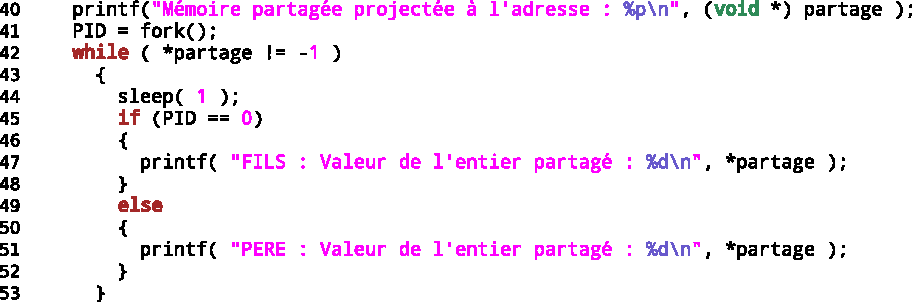
\includegraphics[width=\linewidth]{fig21.pdf}

\titre{Conclusion :} On pouvait naturellement imaginer que les deux processus allaient reconnaitre la valeur de l'entier partagé. En effet, la mémoire est copiée du père au fils, et l'espace mémoire mappé est donc copié avec son mapping, donc dans le fils le mapping vers le fichier virtuel existe toujours. C'est bien ce résultat attendu qui s'est produit. \\

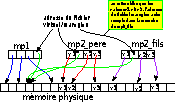
\includegraphics[width=\linewidth]{fig20.pdf}\\


\includegraphics[width=\linewidth]{fig22.pdf}
